\documentclass[12pt,a4paper]{article}

% --------------------------------------------------
% JEZIK IN KODIRANJE
% --------------------------------------------------
\usepackage[utf8]{inputenc}
\usepackage[T1]{fontenc}
\usepackage[slovene]{babel}

% --------------------------------------------------
% POSTAVITEV STRANI
% --------------------------------------------------
\usepackage[a4paper,margin=2.5cm]{geometry}
\usepackage{setspace}
\onehalfspacing

% --------------------------------------------------
% MATEMATIKA
% --------------------------------------------------
\usepackage{amsmath}
\usepackage{amssymb}

% --------------------------------------------------
% TABELE IN GRAFI
% --------------------------------------------------
\usepackage{booktabs}
\usepackage{graphicx}
\usepackage{pgfplots}
\pgfplotsset{compat=1.18}

% --------------------------------------------------
% POVEZAVE
% --------------------------------------------------
\usepackage[hidelinks]{hyperref}

% --------------------------------------------------
% CITIRANJE
% --------------------------------------------------
\usepackage[round,authoryear]{natbib}

% --------------------------------------------------
% ODSTAVKI
% --------------------------------------------------
\setlength{\parindent}{0pt}
\setlength{\parskip}{0.7em}

% --------------------------------------------------
% NASLOV
% --------------------------------------------------
\title{\textbf{Tobinov q kot razmerje med tržno vrednostjo in nadomestitveno vrednostjo}}
\author{}
\date{}

\begin{document}

\maketitle

% ==================================================
\section{Opredelitev Tobinovega q}
% ==================================================

Tobinov q je ekonomski kazalnik, ki povezuje \textbf{tržno vrednost podjetja oziroma njegovega kapitala z nadomestitvenimi stroški tega kapitala}. Njegov osnovni namen je pokazati, kako je vrednost kapitala, kot jo ocenjuje trg, primerljiva s stroškom, ki bi bil potreben za ponovno vzpostavitev oziroma nadomestitev tega kapitala. V najpreprostejši obliki ga lahko zapišemo kot:

\begin{equation}
q =
\frac{\text{tržna vrednost kapitala}}
{\text{nadomestitvena vrednost kapitala}}.
\end{equation}

Pri tem je pomembno razlikovati med \textbf{povprečnim q} in \textbf{mejnim oziroma marginalnim q}. Povprečni q primerja celotno tržno vrednost podjetja oziroma njegovega kapitala s celotno nadomestitveno vrednostjo kapitala. Mejni q pa primerja vrednost \emph{dodatne enote kapitala} z njenim nadomestitvenim stroškom. Prav mejni q je v teoretičnem modelu pomemben za odločanje o novih investicijah. Hayashijeva formalizacija pokaže, da je pod določenimi predpostavkami mogoče marginalni q povezati s povprečnim q, ki ga je v praksi precej lažje opazovati \citep{AndreiMannMoyen2017,PetersTaylor2016}.

Logika kazalnika je relativno preprosta. Če je $q>1$, je tržna vrednost kapitala višja od stroška njegove nadomestitve. To pomeni, da trg podjetju oziroma njegovemu kapitalu pripisuje višjo vrednost, kot bi znašal strošek ustvarjanja primerljivega kapitala. V osnovnem investicijskem modelu to ustvarja spodbudo za dodatne investicije. Če je $q<1$, je situacija obrnjena: tržna vrednost kapitala je nižja od njegove nadomestitvene vrednosti, zato je ekonomska spodbuda za ustvarjanje dodatnega kapitala šibkejša. Pri $q \approx 1$ je tržna vrednost kapitala približno enaka strošku njegove nadomestitve.

Zato lahko Tobinov q razumemo kot \textbf{formalno povezavo med vrednotenjem kapitala in investicijsko odločitvijo}. Ne pove neposredno, ali bo neka investicija uspešna, ampak omogoča primerjavo med vrednostjo, ki jo kapital ustvarja oziroma ji jo pripisuje trg, in stroškom njegovega ustvarjanja.

Pri tem je pomembno, da Tobinov q ni enak klasičnemu računovodskemu kazalniku donosnosti. Ne meri neposredno dobička na vloženi evro in tudi ne predstavlja klasičnega kazalnika ROI. Njegova posebnost je v tem, da na eni strani uporablja \textbf{tržno vrednost}, na drugi pa \textbf{nadomestitveno vrednost kapitala}. V literaturi se Tobinov q zato uporablja kot merilo investicijskih priložnosti podjetja \citep{PetersTaylor2016}.

\begin{table}[htbp]
\centering
\caption{Osnovna interpretacija Tobinovega q}
\label{tab:interpretacija_q}
\begin{tabular}{p{3cm}p{10cm}}
\toprule
\textbf{Vrednost q} & \textbf{Interpretacija} \\
\midrule
$q>1$ &
Tržna vrednost kapitala je višja od nadomestitvenega stroška, zato obstaja večja ekonomska spodbuda za nove investicije. \\

$q\approx1$ &
Tržna vrednost kapitala je približno enaka nadomestitvenemu strošku. \\

$q<1$ &
Tržna vrednost kapitala je nižja od nadomestitvenega stroška, zato je spodbuda za nove investicije šibkejša. \\
\bottomrule
\end{tabular}
\end{table}


% ==================================================
\section{Povezava Tobinovega q z investicijami}
% ==================================================

Povezava med q in investicijami izhaja iz vprašanja, ali se podjetju splača povečati svoj kapital. Če je vrednost dodatnega kapitala na trgu višja od stroška njegovega ustvarjanja, je povečanje kapitala ekonomsko smiselno.

To lahko ponazorimo zelo preprosto. Predpostavimo, da podjetje za vzpostavitev dodatne enote kapitala potrebuje 100 milijonov evrov. Če trg tej dodatni enoti kapitala pripisuje vrednost 120 milijonov evrov, je:

\begin{equation}
q=\frac{120}{100}=1,2.
\end{equation}

Torej je q večji od 1. Če pa bi bila tržna vrednost tega kapitala samo 80 milijonov evrov, bi bil:

\begin{equation}
q=\frac{80}{100}=0,8.
\end{equation}

V prvem primeru je razmerje med tržno vrednostjo in stroškom ustvarjanja kapitala ugodno, v drugem pa ne.

Pri Tobinovem q je zato pomembna predvsem \textbf{mejna vrednost kapitala}. Podjetje se ne odloča samo na podlagi tega, koliko je vreden njegov obstoječi kapital, temveč predvsem na podlagi vprašanja, kakšno vrednost bo ustvarila dodatna investicija. Teorija q investicij predpostavlja povezavo med tržno vrednostjo podjetij in njihovo investicijsko aktivnostjo. Hayashijeva formalizacija je pomembna zato, ker pokaže, pod katerimi pogoji je mogoče marginalni q povezati s povprečnim q, ki ga je  empirično lažje izračunati \citep{AndreiMannMoyen2017}.

To je posebej pomembno pri novih tehnologijah. Pri tehnologiji, kot je umetna inteligenca, investicije niso omejene samo na nakup fizične opreme. Potrebni so tudi podatkovni centri, računalniška oprema, čipi, programska oprema, podatki, raziskave in razvoj ter znanje zaposlenih. Zato je pri AI težje določiti natančno nadomestitveno vrednost kapitala kot pri bolj tradicionalnih oblikah kapitala.

Prav tukaj se pojavi ena izmed pomembnih omejitev uporabe Tobinovega q pri umetni inteligenci.


% ==================================================
\section{Tobinov q in investicije v razvoj umetne inteligence}
% ==================================================

Naša osrednja tema je vprašanje \textit{»Investicije v razvoj umetne inteligence: ali so pričakovanja donosov upravičena?«} Tobinov q nam lahko pri tem pomaga predvsem kot formalni okvir za razumevanje razmerja med velikimi investicijami v AI in vrednostjo, ki jo trgi pripisujejo podjetjem, ki te investicije izvajajo.

V zadnjih letih so investicije v umetno inteligenco zelo hitro naraščale. Stanfordov AI Index za leto 2026 ugotavlja, da je globalna zasebna investicija v AI leta 2025 dosegla približno 344,66 milijarde USD. Skupne investicije, ki vključujejo tudi druge oblike financiranja, so dosegle rekordno raven, pri čemer je bila rast posebej izrazita pri generativni umetni inteligenci \citep{StanfordAIIndex2026}.

To je pomembno za Tobinov q, saj lahko zelo visoke tržne vrednosti AI podjetij razumemo kot znak, da trg pričakuje, da bodo njihove prihodnje dejavnosti ustvarjale veliko vrednost glede na sredstva, ki jih podjetja trenutno gradijo.

Vendar tukaj ne smemo narediti prehitrega sklepa: \textbf{visok q še ne pomeni, da je investicija dejansko donosna}. Pomeni predvsem, da je tržna vrednost kapitala visoka glede na njegovo nadomestitveno vrednost. Če se bodo prihodnji prihodki in produktivnost povečali dovolj, se lahko visoko vrednotenje upraviči. Če se ne bodo, pa lahko pride do zmanjšanja tržne vrednosti in posledično do padca q.

Pri AI je to vprašanje še posebej pomembno, ker se danes veliko investira v infrastrukturo, katere ekonomska korist se bo pokazala šele v prihodnosti. OECD ugotavlja, da so podjetja, povezana z AI infrastrukturo in gostovanjem, leta 2025 prejela približno 109,3 milijarde USD tveganega kapitala. Med letoma 2012 in 2025 je kumulativna investicija v ta segment dosegla približno 256,1 milijarde USD. To kaže na zelo hitro rast investicij v računsko infrastrukturo, ki je potrebna za razvoj in uporabo naprednih sistemov umetne inteligence \citep{OECD2026}.

To pomeni, da trenutno nastaja zelo velika količina novega kapitala, povezanega z AI. Tobinov q je zanimiv zato, ker postavlja vprašanje: \textbf{ali bo prihodnja tržna oziroma ekonomska vrednost tega kapitala dovolj velika, da bo upravičila stroške njegovega ustvarjanja?}

Pri tem se naša tema neposredno poveže z vprašanjem upravičenosti pričakovanih donosov. Če bi prihodnja produktivnost in prihodki zaradi AI dovolj povečali vrednost podjetij, bi bil visok q lahko združljiv z dolgoročno uspešnimi investicijami. Če pa se investicije povečujejo hitreje kot prihodnja ustvarjena vrednost, obstaja možnost, da trenutne vrednosti kapitala niso dolgoročno vzdržne.

Pomemben del tega procesa je tudi povečanje kapitalskih izdatkov za podatkovne centre. Federal Reserve v svojem poročilu o denarni politiki ugotavlja, da je bila rast poslovnih fiksnih investicij v ZDA v veliki meri povezana prav z izgradnjo infrastrukture, potrebne za podporo storitvam umetne inteligence. Od leta 2022 se je močno povečala gradnja novih podatkovnih centrov, skupaj z investicijami v opremo in programsko opremo, ki jih ti centri potrebujejo \citep{FederalReserve2026}.

Tukaj lahko Tobinov q uporabimo kot konceptualni most: \textbf{večje investicije so upravičene, če povečujejo vrednost kapitala dovolj glede na strošek njegovega ustvarjanja}.


% ==================================================
\section{ZDA in Kitajska: dve različni investicijski okolji}
% ==================================================

Tako ZDA kot tudi Kitajske sta državi, ki sodita med vodilnime na področju umetne inteligence, vendar imata precej različne strukture financiranja in investicij.

Podatki Stanfordovega AI Indexa kažejo zelo veliko razliko v zasebnih AI investicijah. Leta 2025 so zasebne investicije v AI v ZDA dosegle približno \textbf{285,88 milijarde USD}, medtem ko so na Kitajskem znašale približno \textbf{12,41 milijarde USD}. ZDA so tako investirale približno 23-krat več zasebnega kapitala kot Kitajska. Stanfordov AI Index pri tem posebej opozarja, da zasebni podatki za Kitajsko verjetno podcenjujejo njeno celotno AI porabo, saj ima pomembno vlogo tudi državno usmerjanje kapitala \citep{StanfordAIIndex2026}.

\begin{figure}[htbp]
\centering
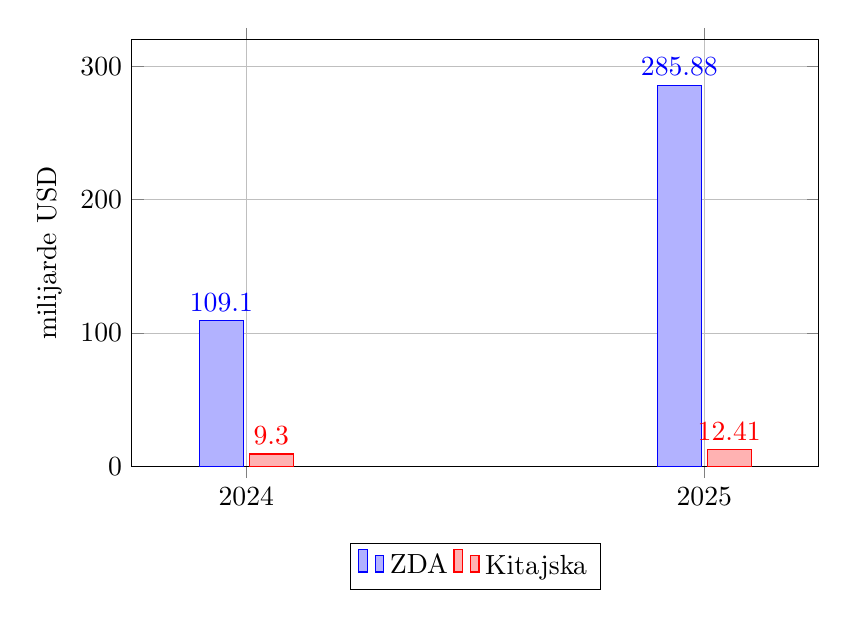
\begin{tikzpicture}
\begin{axis}[
    ybar,
    bar width=16pt,
    width=0.85\textwidth,
    height=7cm,
    ylabel={milijarde USD},
    symbolic x coords={2024,2025},
    xtick=data,
    ymin=0,
    ymax=320,
    legend style={at={(0.5,-0.18)},anchor=north,legend columns=2},
    nodes near coords,
    nodes near coords align={vertical},
    enlarge x limits=0.25,
    grid=major,
]
\addplot coordinates {(2024,109.10) (2025,285.88)};
\addplot coordinates {(2024,9.30) (2025,12.41)};
\legend{ZDA, Kitajska}
\end{axis}
\end{tikzpicture}
\caption{Zasebne investicije v umetno inteligenco v ZDA in na Kitajskem, 2024--2025.}
\label{fig:us_china_ai}
\end{figure}

\noindent
\textit{Vir podatkov: Stanford HAI, AI Index Report 2026 \citep{StanfordAIIndex2026}.}

Vendar bi bilo napačno iz tega neposredno sklepati, da Kitajska v AI investira 23-krat manj. Stanford opozarja, da zasebni podatki za Kitajsko ne zajamejo v celoti državnega financiranja. Kitajski državni oziroma usmerjevalni skladi so med letoma 2000 in 2023 v AI podjetja usmerili ocenjenih \textbf{184 milijard USD}. Zato je pri primerjavi ZDA in Kitajske zelo pomembno razlikovati med \textbf{zasebnim investiranjem} in \textbf{celotnimi investicijami v AI} \citep{StanfordAIIndex2026}.

Podobno razliko pokažejo podatki OECD. Ameriška podjetja so leta 2025 predstavljala približno \textbf{75 \% svetovne vrednosti AI poslov tveganega kapitala}, medtem ko je Kitajska predstavljala približno 5 \%. ZDA so bile tako daleč največji prejemnik AI tveganega kapitala. Vrednost AI poslov tveganega kapitala v ameriških podjetjih je dosegla približno 194 milijard USD, kitajskih podjetij pa približno 13,9 milijarde USD \citep{OECD2026}.

\begin{figure}[htbp]
\centering
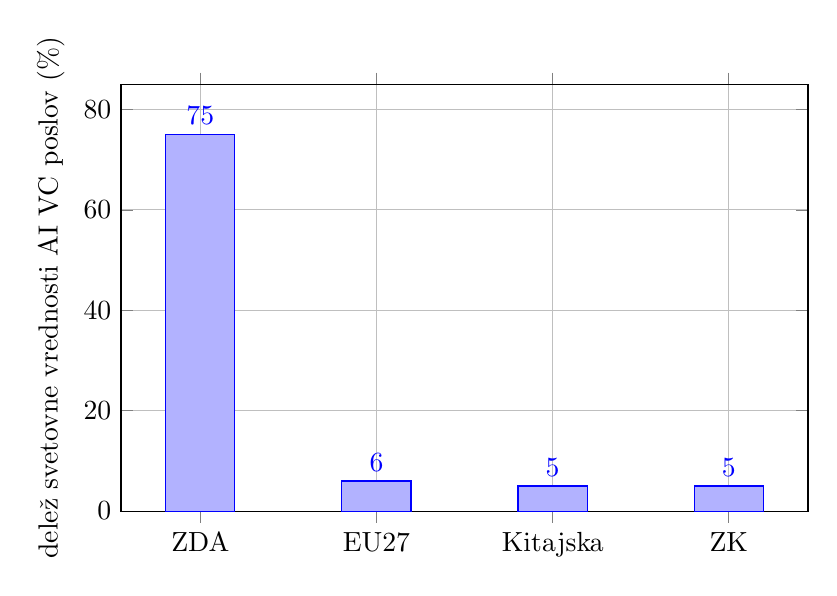
\begin{tikzpicture}
\begin{axis}[
    ybar,
    bar width=25pt,
    width=0.85\textwidth,
    height=7cm,
    ylabel={delež svetovne vrednosti AI VC poslov (\%)},
    symbolic x coords={ZDA,EU27,Kitajska,ZK},
    xtick=data,
    ymin=0,
    ymax=85,
    nodes near coords,
    nodes near coords align={vertical},
    enlarge x limits=0.15,
    grid=major,
]
\addplot coordinates {
    (ZDA,75)
    (EU27,6)
    (Kitajska,5)
    (ZK,5)
};
\end{axis}
\end{tikzpicture}
\caption{Delež svetovne vrednosti AI poslov tveganega kapitala v letu 2025.}
\label{fig:vc_share}
\end{figure}

\noindent
\textit{Vir podatkov: OECD, \textit{Venture capital investments in artificial intelligence through 2025} \citep{OECD2026}.}

To je pomembno tudi z vidika Tobinovega q. Pri ZDA je velik del financiranja povezan z zasebnimi podjetji in kapitalskimi trgi, zato se lahko tržna vrednost podjetij relativno neposredno povezuje z njihovimi investicijami. Pri Kitajski pa je vlogo države težje ločiti od tržnega financiranja. Zato je neposredna primerjava Tobinovega q med obema državama metodološko zahtevna.


% ==================================================
\section{Zakaj je Tobinov q pri AI posebej zanimiv, vendar tudi omejen}
% ==================================================

Pri umetni inteligenci se pojavi še en pomemben problem: \textbf{nadomestitvena vrednost kapitala ni enostavno določljiva}.

Pri fizičnem stroju lahko relativno jasno določimo, koliko bi stalo kupiti nov stroj z enakimi ali podobnimi značilnostmi. Pri AI pa je velik del kapitala neopredmeten. Podjetje lahko investira v programsko opremo, podatke, algoritme, raziskave, znanje zaposlenih in organizacijske spremembe. Del teh investicij ni nujno v celoti prikazan kot fizični kapital v računovodskih podatkih.

To pomeni, da lahko pri izračunu q dobimo razmeroma visoko razmerje tudi zato, ker je \textbf{imenovalec -- nadomestitvena vrednost kapitala -- podcenjen glede na dejansko količino ustvarjenega neopredmetenega kapitala}.

Ta problem je posebej pomemben za tehnološka podjetja. Peters in Taylor ugotavljata, da vključitev neopredmetenega kapitala izboljša razumevanje povezave med Tobinovim q in investicijami. Njuna analiza pokaže, da Tobinov q po vključitvi neopredmetenega kapitala bolje pojasnjuje tako fizične kot neopredmetene investicije, pri čemer je povezava posebej pomembna pri podjetjih, kjer ima neopredmeteni kapital večjo vlogo \citep{PetersTaylor2016}.

To je neposredno relevantno za umetno inteligenco, saj so podatki, programska oprema, raziskave in razvoj ter organizacijsko znanje pomemben del AI investicij. Če jih merimo samo preko tradicionalnega fizičnega kapitala, lahko dobimo nepopolno sliko dejanske investicijske osnove podjetja.

Prav zato je pri AI klasični Tobinov q najbolje uporabljati kot \textbf{analitični okvir}, ne kot popoln samostojen dokaz donosnosti.

Raziskava Andreija, Manna in Moyena prav tako opozarja na problem merjenja neopredmetenega kapitala. Avtorji ugotavljajo, da so raziskovalno intenzivne panoge in podjetja z več neopredmetenega kapitala pomemben primer, pri katerem lahko klasično merjenje Tobinovega q povzroča težave, vendar hkrati ugotavljajo, da je povezava med q in investicijami v takšnih podjetjih lahko zelo pomembna \citep{AndreiMannMoyen2017}.

Če danes opazujemo zelo visoke investicije v AI, še ne pomeni nujno, da je donosnost nizka samo zato, ker trenutna produktivnost še ni tako visoka. Del koristi se lahko pojavi šele po tem, ko podjetja prilagodijo svoje procese in začnejo AI dejansko uporabljati v proizvodnji in storitvah.


% ==================================================
\section{Kaj nam Tobinov q pove o upravičenosti investicij v AI?}
% ==================================================

Tobinov q nam zato ne more dati enostavnega odgovora \textit{»da« ali »ne«} na vprašanje, ali so pričakovanja donosov od AI upravičena. Lahko pa nam da jasen formalni okvir za razmišljanje o tem vprašanju.

Prvič, če je tržna vrednost podjetij, ki intenzivno investirajo v AI, bistveno višja od nadomestitvene vrednosti njihovega kapitala, je q visok. To je skladno z idejo, da trg pričakuje visoko prihodnjo vrednost tega kapitala. Takšno vrednotenje je lahko upravičeno, če bodo AI investicije povzročile dovolj visoko rast prihodkov, produktivnosti in prihodnjih denarnih tokov.

Drugič, visoke investicije same po sebi še ne dokazujejo visoke donosnosti. Če podjetja gradijo velike količine podatkovnih centrov in kupujejo drago računalniško infrastrukturo, mora biti prihodnja uporaba te infrastrukture dovolj velika, da upraviči stroške. Federal Reserve ugotavlja, da je bila v ZDA rast kapitalskih izdatkov v zadnjem obdobju močno povezana prav z gradnjo infrastrukture za AI \citep{FederalReserve2026}.

Tretjič, pri primerjavi ZDA in Kitajske moramo biti previdni. ZDA imajo bistveno več zasebnih AI investicij in izrazito razvite kapitalske trge, medtem ko ima Kitajska večjo vlogo države pri usmerjanju kapitala. Zato razlika v zasebnih investicijah ne pomeni nujno enake razlike v skupni količini kapitala, namenjenega AI.

Četrtič, pri AI je posebej pomemben problem merjenja. Če del ustvarjenega kapitala predstavljajo podatki, programska oprema, organizacijsko znanje in človeški kapital, potem klasični izračun Tobinovega q ne zajame nujno celotne ekonomske vrednosti investicije. Zato je pri AI q najbolje uporabljati kot \textbf{formalni merilni okvir}, ne kot popoln samostojen kazalnik donosnosti.


% ==================================================
\section{Sklep}
% ==================================================

Tobinov q je uporaben zato, ker na relativno preprost način poveže \textbf{tržno vrednost kapitala z njegovim nadomestitvenim stroškom}. Njegova osnovna logika je, da q nad 1 kaže na razmere, v katerih je vrednost kapitala višja od stroška njegovega ustvarjanja, kar je povezano z večjo spodbudo za nove investicije. Pri q pod 1 je ta spodbuda šibkejša. Formalna povezava med q in investicijami je posebej pomembna pri marginalnem q, ki se nanaša na vrednost dodatne enote kapitala \citep{AndreiMannMoyen2017,PetersTaylor2016}.

Za našo temo je Tobinov q zanimiv predvsem zato, ker omogoča razmislek o tem, \textbf{ali so ogromne investicije v umetno inteligenco podprte z dovolj veliko pričakovano ekonomsko vrednostjo}. ZDA so trenutno daleč največji zasebni investitor v AI, medtem ko je Kitajska po zasebnih investicijah precej za njimi. Hkrati pa kitajski podatki vključujejo pomembno vlogo državnega financiranja, zato sama primerjava zasebnih investicij ne predstavlja celotne slike \citep{StanfordAIIndex2026}.

Prav tu je glavna povezava z našim raziskovalnim vprašanjem. \textbf{Če visoke investicije v AI vodijo do dovolj velikega povečanja prihodnje produktivnosti, prihodkov in vrednosti kapitala, so lahko visoka vrednotenja in visoke investicije dolgoročno upravičeni. Če pa se nadomestitveni stroški kapitala povečujejo hitreje od njegove dejanske ekonomske vrednosti, se lahko pokaže, da so bile investicije glede na ustvarjeno vrednost previsoke.}

Pri tem pa je treba upoštevati posebnost AI: njen kapital ni samo fizičen. Podatki, programska oprema, znanje zaposlenih in organizacijske spremembe predstavljajo pomemben del investicije, vendar jih je težje vključiti v klasično merjenje kapitala. Zato Tobinov q pri AI ni popoln merilni instrument, je pa zelo uporaben \textbf{formalni okvir za primerjavo velikosti investicij, vrednotenja kapitala in pričakovane prihodnje ekonomske vrednosti} \citep{PetersTaylor2016}.

V primeru ZDA in Kitajske je zato bolj smiselno vprašati, \textbf{kako se razlikujeta struktura investicij in financiranja AI ter ali se visoke investicije odražajo tudi v ustvarjeni ekonomski vrednosti}, kot pa preprosto zaključiti, da država, ki investira več, nujno dosega višji donos. To omogoča bolj previden in ekonomsko utemeljen odgovor na vprašanje, ali so pričakovanja glede donosov od umetne inteligence upravičena.

\end{document}